\chapter{Analysis}

\section{Datasets}
è iortante dei dire che sono stati utilizzati due datasets.
The labeled datasets employed in the ensuing analysis are all products of Monte Carlo simulation, generated via the SNiPER software.

The first of the datasets provided is specifically tailored for the study of Inverse Beta Decay (IBD) events. Each event within this dataset, simulated and injected into the system, is tagged with a unique Simulation Identifier, or SimID. Furthermore, events which trigger a sufficient number of PMTs to be captured by the electronic system are assigned an EventID. This intricate labeling system allows for a clear differentiation between correlated IBD events, which represent actual IBD occurrences, and uncorrelated IBD events.


The second dataset focuses primarily on radioactivity events. Similar to the IBD dataset, it encompasses a large number of simulated events, each reflecting the complex reality of real-world physics phenomena. Additionally, the inherent electronic noise prevalent in actual physical environments is accurately accounted for, ensuring a realistic representation within the simulated context.

In this research undertaking, my central task will focus on a detailed examination and evaluation of the provided datasets. My work will primarily involve not just interpreting the inherent characteristics and peculiarities of the recorded events, but also harnessing these insights to construct comprehensive feature tables. These feature tables, generated from the datasets, will serve as the basis for my subsequent analysis and interpretation, a process which will be elaborated upon in the following sections of this study. The aim is to provide a meaningful understanding of the correlations and implications of these events within the broader context of the JUNO experiment.

%TODO-> Inserire il fatto che i dataset sono stati creati in ordine temporale in parallelo con SimID Per simulare 1500000 eventi nel MonteCarlo ci vorrebbero mesi e mesi di tempo macchina.
%Per affrontare il problema, si parallelizza la simulazione su una infrastruttura chiamata DCI (Distributed Computing Infrastructure).
%In questo modo si può ad esempio dividere i 1500000 eventi in 1500 jobs (simulati quindi da 1500 CPU diverse) da 1000 event ciascuno, completando la produzione in poche ore invece che in mesi.
%Questo approccio ha però il drawback che ogni simulazione parallela sarà indipendente dalle altre e quindi per ciascuna di queste il tempo, i SimID e tutte le altre quantità partirano da 0"" 

%La seconda colonna -> Si, sono il numero di eventi generati. Non tutti gli eventi generati interagiscono con il detector: un evento generato nella struttura metallica può venire fermato nella struttura stessa e non interagire con il detector, o ancora un evento generato nell'acrilico può venire emesso verso l'esterno e quindi non entrare mai in contatto con il detector e così via.
%Se consideri ora solo gli eventi che davvero sono entrati in contatto con il detector, non tutti gli eventi vengono ricostruiti: alcuni eventi sono così poco energetici che non sono sufficienti ad illuminare i PMT e quindi ad azionare il trigger per l'acquisizione dell'evento.

%Per darti un'idea, la rate di decadimenti radioattivi è circa 6.6 MHz, ne vengono effettivamente registrati dal detector appena 100 Hz (o poco meno)

%Questa è una delle sfide più grandi, perchè devi portare un segnale di circa 100 Hz (8.6 x 10e6 eventi/giorno) a rappresentare meno di 1 evento/giorno di background
%-------------------

%Nel MonteCarlo sono inclusi tutti gli effetti che ci aspettiamo nella realtà. E purtroppo, nella realtà, l'elettronica ha un rumore intrinseco (ad esempio puoi cercare in letteratura il Dark Count Rate per i PMTs).
%Ora, nel MonteCarlo vengono iniettati degli eventi (ad esempio una coppia prompt-delayed da IBD). A questo evento iniettato viene associato un SimID (simulation identifier) incrementale. Siccome prompt e delayed sono stati iniettati assieme, avranno lo stesso SimID.
%Non tutti gli eventi però sono registrati e salvati dall'elettronica. In JUNO, un evento viene salvato solo se questo è in grado di illuminare nello stesso momento un gran numero di PMTs (corrispondenti a qualche centinaio di keV).
%Se questo avviene, viene generato un trigger, viene salvato l'evento e gli viene associato un EventID incrementale.
%Può succedere che, per puro caso, il rumore intrinseco dell'elettronica "accenda" nello stesso momento un gran numero di PMT. In questo caso, nessun evento vero di fisica ha generato questo trigger, ma l'elettronica acquisisce e salva comunque questo evento, perch`ha superato la soglia di trigger. Quello che succede in questo caso è che l'evento avrà un EventID, ma nessun SimID associato, perchè nessun evento è stato davvero iniettato nella simulazione.
%Al contrario, può succedere che tu inietti una certa particella a cui quindi viene associato un SimID), ma questa non riesce a illuminare abbastanza PMT, l'evento non viene salvato e quindi non gli viene associato nessun EventID e non viene salvato nel file finale.


%Prima coppia simulata si becca SimID di 0. Gli Event IDs associati saranno 0 e 1.
%Seconda coppia generata avrà SimID di 1. EventIDs in questo caso sarnno 2 e 3. Ecc ecc.
%Sono incrementali per convenzione.

%TODO-> Spiega cosa c'è nei datasets -- ['EventID', 'SimID', 'timestamp', 't_sec', 't_nanosec', 'recx', 'recy', 'recz', 'm_QEn', 'm_pe']
%TODO-> Mention unbalanced datasets problem


%Ciao Fabio, la radioattività con cui hai lavorato rappresenta tutto il contributo da decadimenti radioattivi (alfa, beta, gamma) interno ed esterno a detector, ma che hanno depositato energia all'interno del detector.Ti lascio la tabella degli isotopi e delle rate di decadimento generate qui di seguito:

 

\begin{table}[htp]
\centering
\begin{tabular}{|c|c|c|}
	\hline
 \textbf{Dataset Name}  & \textbf{Number of Events}  & \textbf{Rates (used in elecsim)}   \\\hline\hline
      U238@LS      &   1,000,000 events    &           3.234 Hz            \\\hline
     Th232@LS      &   1,000,000 events    &           0.733 Hz            \\\hline
      K40@LS       &   1,000,000 events    &           0.53 Hz             \\\hline
     Pb210@LS      &   1,000,000 events    &           17.04 Hz            \\\hline
      C14@LS       & 1,000,000,000 events  &           3.3e4 Hz            \\\hline
      Kr85@LS      &   1,000,000 events    &           1.163 Hz            \\\hline
   U238@Acrylic    &   10,000,000 events   &           98.41 Hz            \\\hline
   Th232@Acrylic   &   10,000,000 events   &           22.29 Hz            \\\hline
    K40@Acrylic    &   10,000,000 events   &          161.25 Hz            \\\hline
   U238@node/bar   &  100,000,000 events   &          2102.36 Hz           \\\hline
  Th232@node/bar   &  100,000,000 events   &          1428.57 Hz           \\\hline
   K40@node/bar    &  100,000,000 events   &           344.5 Hz            \\\hline
   Co60@node/bar   &  100,000,000 events   &           97.5 Hz             \\\hline
   U238@PMTGlass   & 1,000,000,000 events  &          4.90e6 Hz            \\\hline
  Th232@PMTGlass   & 1,000,000,000 events  &          8.64e5 Hz            \\\hline
   K40@PMTGlass    & 1,000,000,000 events  &          4.44e5 Hz            \\\hline
  Tl208@PMTGlass   & 1,000,000,000 events  &          1.39e5 Hz            \\\hline
    Co60@Truss     &           0           &             ? Hz              \\\hline
    Tl208@Truss    &           0           &             ? Hz              \\\hline
 Rn222@WaterRadon  &  100,000,000 events   &            90 Hz              \\\hline
\end{tabular}
\caption{Here Caption}
\label{tab:BKG_gen}
\end{table}

\newpage

\section{Feature creation}
%TODO: devi sppiegare che il codice è satao runnato su cloudveneto che mi semvra tu non l'abbia mai specifiato.

The development of machine learning models for the detection of Inverse Beta Decay (IBD) events necessitates a systematic and efficient approach to feature engineering. This process begins with the loading of two separate datasets, one for IBDs and one for radioactivity background, each containing a multitude of potential IBD events. The primary objective is to construct a feature table that encapsulates the unique characteristics of these events, providing a robust foundation for subsequent model training.

\subsection{IBD dataset}
As we mentioned earlier, an IBD event is characterized by two distinct signals with different energies, positions, and times. The first, known as the prompt signal, is caused by the annihilation of a positron with an electron in the scintillator liquid. This interaction yields a signal with a characteristic energy. The second, the delayed signal, results from the capture of a neutron by the scintillator liquid. This signal occurs with a significant delay, at a different position, and with a different energy compared to the prompt signal.

To create the feature table, all possible pairs of events within the dataset were considered, without repetition. Each possible combination was ordered temporally, meaning the second event followed the first. This temporal ordering is crucial in feature determination. Given a pair $i-j$, and considering that neutron capture occurs temporally subsequent to electron-positron annihilation, the following features were constructed:


\begin{itemize}
	 
	\item \textbf{$R_{prompt}$}: This feature represents the distance of the prompt signal, calculated as the distance from the origin to the point $(x_i, y_i, z_i)$ in the detector space where the prompt signal occurred.	
	
	\item $R_{delayed}$: Similar to $R_{prompt}$, this feature represents the distance of the delayed signal, calculated as the distance from the origin to the point $(x_j, y_j, z_j)$ in the detector space where the delayed signal occurred.

	\item \textbf{$E_{prompt}$}: This feature represents the energy of the prompt signal. It captures the characteristic energy released during the annihilation of a positron with an electron in the scintillator liquid.

	\item \textbf{$E_{delayed}$}: This feature represents the energy of the delayed signal. It captures the energy released when a neutron is captured by the scintillator liquid. This capture can occur by hydrogen, resulting in a gamma ray with an energy of approximately 2.2 MeV, or by carbon, resulting in gamma rays with combined energies of about 4.95 MeV to 5.12 MeV.

	\item \textbf{$\Delta_{Time}$}: This feature represents the time difference between the two events. It captures the temporal delay between the occurrence of the prompt and delayed signals.

	\item \textbf{$\Delta_{Radius}$}: This feature represents the spatial distance between the two events. It captures the spatial separation between the points in the detector space where the prompt and delayed signals occurred.

\end{itemize}
These features encapsulate the temporal and spatial differences between the prompt and delayed signals, as well as their respective energies, providing a comprehensive representation of the unique characteristics of IBD events.


\subsubsection*{Event Labeling}

In the context of supervised learning, the process of labeling is crucial as it provides the ground truth against which the performance of the machine learning model is evaluated. In this scenario, each pair of events in the dataset is assigned a label that indicates whether it represents a true Inverse Beta Decay (IBD) event or a background signal (BKG).

The label is a binary value: a label of 1 signifies a true IBD event, while a label of 0 signifies a BKG event. The assignment of these labels is not arbitrary but is guided by a specific criterion based on the simulation identifier (SimID) associated with each event pair.

The SimID is a unique identifier assigned to each simulated event pair during the generation of the dataset. If a pair of events share the same SimID, it means they were generated as part of the same simulation and thus are considered to represent a true IBD event. In this case, they are assigned a label of 1.

Conversely, if a pair of events do not share the same SimID, it means they were generated as part of different simulations. These events are not correlated and thus are considered to represent BKG events. In this case, they are assigned a label of 0.

This labeling strategy based on the SimID ensures a systematic and consistent methodology for event classification. It provides a clear and objective criterion to distinguish between true IBD events and BKG events, which is essential for the training and evaluation of the machine learning model.


\subsubsection*{Efficient Feature Calculation}
Given the large size of the dataset and the computational complexity of feature calculation, a parallel computing approach was adopted to enhance efficiency. The feature calculation task was divided into multiple sub-tasks that could be executed simultaneously by different cores of a CPU. This parallelization significantly reduced the total computation time, particularly beneficial when working with large volumes of data.
%TODO: scrivi che il codice è stato scritto per far si che fosse thread safre, cercando evitare il problema dell...

To further optimize the computation, a method was implemented to only consider event pairs where the delayed event occurs within a time window of $5*\tau$ from the prompt event. This approach is based on the fact that the time delay between the prompt and delayed events in Inverse Beta Decay (IBD) typically follows an exponential distribution, a characteristic of radioactive decay processes. While this method significantly reduces the number of potential event pairs, it might exclude about $0.7\%$ of IBD events that occur outside this time window. 

While this percentage is relatively small, it's important to consider the potential impact on the analysis results.

\subsection{Radioactivity dataset}
For the radioactivity dataset, the feature calculation was performed in a manner analogous to the IBD dataset. The key difference is that event pairs from the radioactivity dataset are labeled as BKG events, hence assigned a label of 0.

%TODO: fai una descrizione delle features

\begin{figure}[h]
	\centering
	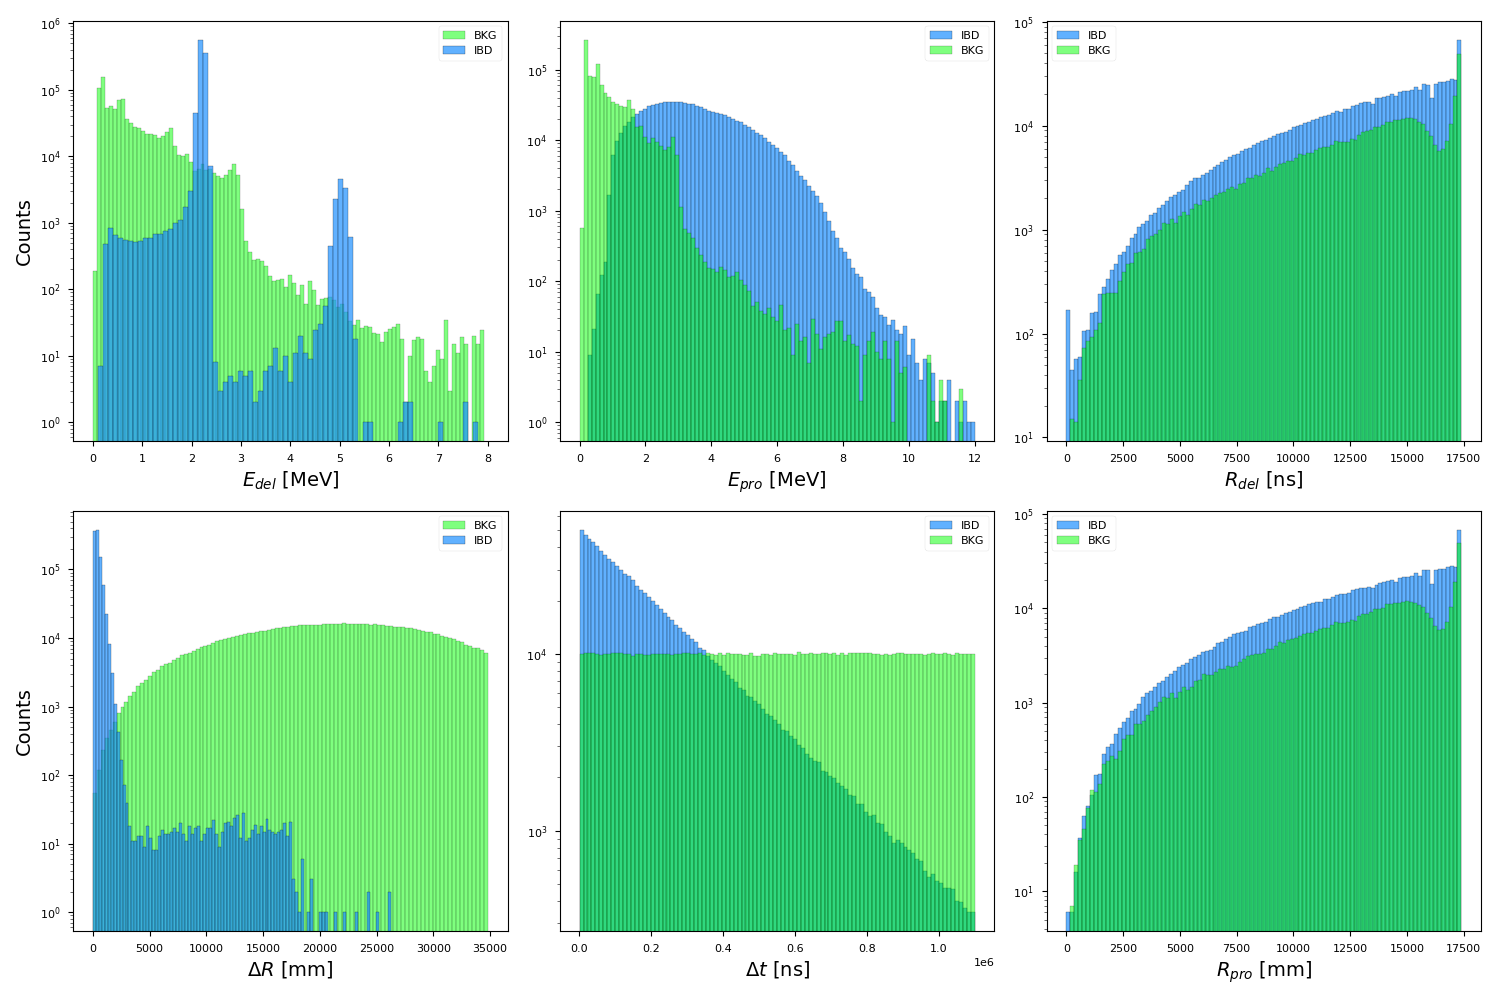
\includegraphics[width=1\linewidth]{Images/hist_features.png}
	\caption{Features histograms}
	\label{fig:hist_features}
\end{figure}



In summary, the feature engineering process for IBD event detection involves careful consideration of the unique characteristics of these events, systematic feature construction, and efficient computation strategies. This process provides a robust foundation for the development and training of machine learning models for IBD event detection.

\section{Models}
In the context of the JUNO experiment, a significant part of the effort involves the implementation and optimization of an event selection algorithm. The primary objective of this algorithm is to identify and select Inverse Beta Decay events induced by reactor antineutrinos, which are of paramount importance in the study of neutrino oscillations.

In this chapter, we will present several algorithms for event selection.\\
 
 The first algorithm is a manual cut-based approach, \textbf{Manual Cut}, where specific cuts are defined to select events of interest. This approach involves setting criteria based on the physical characteristics of the events and known background noise sources in the detector. The manual cut algorithm allows for precise control over the selection process and enhances the signal-to-background ratio.

In addition to the manual cut algorithm, other algorithms discussed in this chapter are based on machine learning models, specificaly based on \textbf{Boosted Decision Trees} and on \textbf{Neural Network}. 

The inclusion of machine learning algorithms in event selection provides an alternative approach that can adapt to complex and evolving data patterns. These algorithms can uncover subtle features in the data that may not be easily captured by manual cuts alone.

By exploring both manual cut and machine learning-based algorithms, we aim to provide a comprehensive understanding of different approaches to event selection, highlighting their strengths and limitations in the context of the JUNO experiment.

\subsection{Manual Cut}
The algorithm is designed to suppress various types of background noise while maintaining high efficiency for true IBD events. The selection criteria, or "cuts", are implemented using Python, and are applied to the Features Tables discussed above. Each cut within the algorithm serves a distinct purpose in the overall event selection process.

The key components of the event selection algorithm are as follows:

\begin{enumerate}
	\item \textbf{Delta Time ($\Delta t$) and Delta Radius ($\Delta R$) cuts}: The first cut is applied on the time delay and the radial distance between the prompt and delayed signals. The criteria are:
	\begin{itemize}
		\item Time separation between the prompt and delayed signals should be less than 1.0 ms.
		\item Spatial 3D separation should be less than 1.5 m.
	\end{itemize}

	These cuts are designed to reduce accidental background noise, which is the coincidence of two otherwise uncorrelated events, typically of radiogenic origin. The accidental background can be measured with excellent precision and subtracted by off-time window techniques. By imposing a limit on the time and spatial separation between the prompt and delayed signals, the algorithm can effectively distinguish between true IBD events and accidental coincidences.
	
	\vspace{-1\baselineskip}

	\begin{figure}[h!]
		\centering
		\subfloat[$\Delta R$ cut]{
			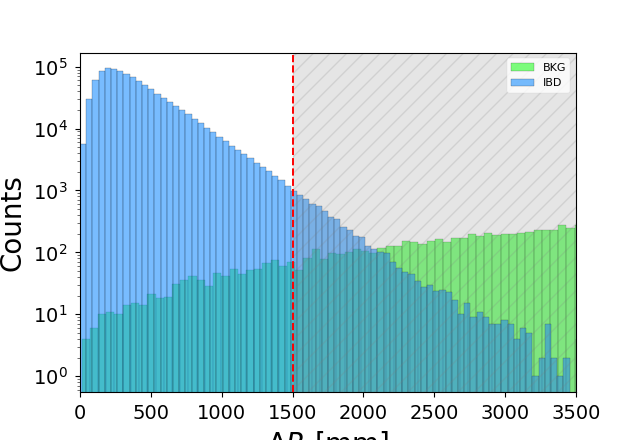
\includegraphics[width=7cm]{Images/Cut/delta_radius.png}
			\label{fig:delta_radius_cut}
		}
		\subfloat[$\Delta t$ cut]{
			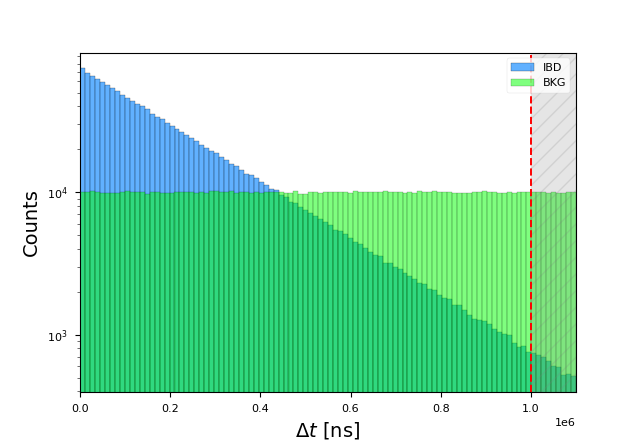
\includegraphics[width=7cm]{Images/Cut/delta_time.png}
		}
		
	\end{figure}
	\vspace{-1\baselineskip}

	\item \textbf{Energy of the Prompt Signal ($E_{pro}$) Cut}: The next cut is applied on the energy of the prompt signal, which is the initial signal produced by the antineutrino interaction. The criteria are:
	\begin{itemize}
		\item Energy of the prompt signal should be within the [0.7, 12.0] MeV range.
	\end{itemize}
	
	\begin{adjustbox}{minipage={\linewidth}, valign=t}
		
		\begin{wrapfigure}{t}{0.5\linewidth}
			
			\vspace{-1\baselineskip}
			\caption{$E_{pro}$ cut}
			\vspace{-0.5\baselineskip}
			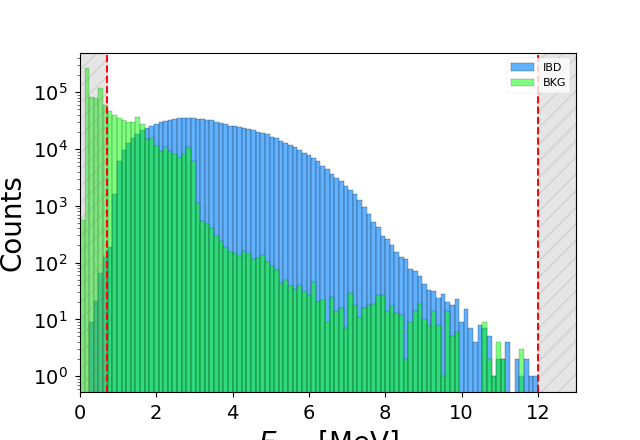
\includegraphics[width=7.5cm]{Images/Cut/e_pro.png}
			\label{fig:e_pto_cut}
			\vspace{-0.2\baselineskip}
			\vspace{-5\baselineskip}
			
		\end{wrapfigure}
		
		\vspace*{0.15em}
		
		This cut is based on the expectation that IBD events dominate this energy range. The energy of the prompt signal corresponds to the energy of the positron from the IBD reaction, and the specific range is chosen to maximize the signal-to-background ratio.\\
		\\
		\newline
		\newline
		
	\end{adjustbox}


	\item \textbf{Energy of the Delayed Signal ($E_{del}$) Cut}: The final cut is applied on the energy of the delayed signal, which is the signal produced by the neutron capture that follows the antineutrino interaction. The criteria are:
	\begin{itemize}
		\item Energy of the delayed signal should be within the [1.9, 2.5] MeV or [4.4, 5.5] MeV ranges.
	\end{itemize}
	
	\begin{adjustbox}{minipage={\linewidth}, valign=t}
		
		\begin{wrapfigure}{t}{0.5\linewidth}
			
			\vspace{-1.5\baselineskip}
			\caption{$E_{del}$ cut}
			\vspace{-0.5\baselineskip}
			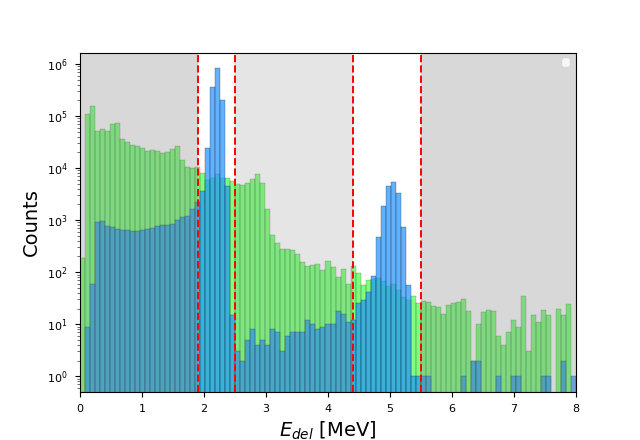
\includegraphics[width=7.5cm]{Images/Cut/e_del.png}
			\label{fig:e_del_cut}
			\vspace{-0.2\baselineskip}
			\vspace{-5\baselineskip}
			
		\end{wrapfigure}
		
		\vspace*{0.15em}
		
		These energy selection windows correspond to neutron capture on hydrogen and carbon, respectively. The energy of the delayed signal is characteristic of the neutron capture process, and the specific ranges are chosen to correspond to the expected energies of neutron capture on hydrogen and carbon in the detector.\\
		\\
		\newline
		\newline
		
	\end{adjustbox}

\end{enumerate}

An evaluation was conducted to assess the accuracy of the algorithm. In this evaluation, the feature table of true IBD events was utilized to gauge the algorithm's performance. The results indicated that out of a total of 1,468,385 events, 1,435,115 events were accurately classified as IBD. This achievement translates to an accuracy rate of $97.73\%$, indicating the algorithm's successful identification of the majority of true IBD events.\\


Furthermore, the efficiency calculation was performed on the background dataset, yielding the following results: 26.0 out of 993,457 events were mistakenly classified as IBD, resulting in an efficiency rate of $99.997\%$. This indicates that the algorithm has an excellent capability to distinguish and reject background events, achieving a high level of efficiency in identifying true IBD events. The extremely low misclassification rate of background events as IBD further highlights the algorithm's effectiveness in minimizing false positives and maintaining a high level of purity in the selected IBD events.
       

A summary table presents the results obtained from the evaluations:

\begin{table}[ht]
	\centering
	\caption{Summary of Algorithm Performance}
	\label{tab:algorithm-results}
	\begin{tabular}{|c|c|c|c|}
		\hline
		Dataset & Total Events & IBD Events Selected & Accuracy (\%) \\ \hline\hline
		True IBD Events & 1,468,385 & 1,435,115 & 97.73 \\ \hline
		Background Events & 993,457 & 26 & 99.997 \\ \hline
	\end{tabular}
\end{table}

\subsection{XGBoost}

%TODO: Cofusion Matrix, Interpretation (Features importance, violin plots, )

In this section, we will delve into the application of the Extreme Gradient Boosting, or XGBoost model, for our event selection task. XGBoost is an advanced and highly efficient implementation of gradient-boosting decision trees, crafted with an emphasis on speed and performance. It uniquely combines the strengths of gradient boosting with the advantages of parallel processing. The result is a powerful, flexible, and fast algorithm that has won favor in a wide range of machine learning tasks and competitions. The speed, performance, and the ability to manage complex patterns of XGBoost make it particularly suited for the event selection in the context of the JUNO experiment. In the following subsections, we will discuss the specifics of how the XGBoost model was developed, optimized, and applied to our task.

The XGBoost model was initialized with several specific hyperparameters to fine-tune the model's performance. These hyperparameters are key factors that determine how the model learns from the data:

\begin{itemize}
	\item  \textbf{Number of parallel threads ($nthread$)} : This hyperparameter is set to -1, which means that the model uses the maximum number of threads available on the system. The number of threads refers to the number of operations that can be run in parallel during training, and using more threads can speed up the training process.
	\item  \textbf{Random seed ($seed$)} : The seed is set to 1 for reproducibility. The seed value is used to initialize the random number generator, which is part of the stochastic aspect of the gradient boosting algorithm. Using the same seed value ensures that the same sequence of random numbers is generated each time the code is run, which allows the results to be reproduced exactly.
	\item  \textbf{Number of estimators ($n_{estimators}$)} : The model was configured with 10,000 estimators. In the context of gradient boosting, an estimator is a single decision tree. The number of estimators represents the maximum number of decision trees to be built, and it is one of the most important hyperparameters to tune. Having more trees makes the model more complex and can lead to better performance on the training data, but if too many trees are used, the model may overfit the training data and perform poorly on unseen data.
	\item  \textbf{Learning rate ($learning_rate$)} : The learning rate was set to 0.05. This hyperparameter controls how much each tree contributes to the final prediction. A smaller learning rate means that each tree has less influence, so more trees are needed to create a model of similar complexity. A smaller learning rate can make the model more robust to overfitting and allow it to generalize better to unseen data.
	\item  \textbf{Maximum tree depth ($max_depth$)} : The maximum depth of each tree was set to 3. The depth of a tree is the length of the longest path from the root to a leaf, and it controls how complex each tree can be. A larger depth allows the model to fit the data more closely, but it can lead to overfitting if the depth is too large. 
\end{itemize}
The chosen hyperparameters strike a balance between computational efficiency and model performance, allowing control over the learning process and model complexity. To optimize the XGBoost model, a Grid Search technique was used. This method systematically evaluated various hyperparameter combinations to identify the optimal configuration that maximizes model accuracy.



\subsubsection{Results}
In this study, we utilized the XGBoost algorithm to classify true Inverse Beta Decay (IBD) events and measure its performance against a dataset of these events. Out of a total of 1,468,385 events, the XGBoost algorithm managed to accurately identify 1,468,344 IBD events. This result corresponds to an impressive efficiency rate of $99.9972\%$, highlighting the superior ability of the XGBoost algorithm to correctly identify the majority of true IBD events.

Further evaluation of the algorithm's performance was conducted on the background dataset. Out of 993,457 background events, only 15 were incorrectly classified as IBD events. This achievement translates to an exceptional efficiency rate of $99.9985\%$. It is clear from these results that the XGBoost algorithm is highly proficient in distinguishing and rejecting background events, achieving a remarkable level of efficiency in identifying true IBD events. The exceptionally low misclassification rate of background events as IBD underlines the effectiveness of the XGBoost algorithm in minimizing false positives in the selected IBD events. 


In addition to previous model evaluations, a confusion matrix was calculated. This provided further insight into the precision and effectiveness of the model. The analysis was applied to a test dataset, representing $20\%$ of the initial dataset of approximately one million elements. The detailed results are illustrated in the Table \ref{tab:conf_matrix_xgb}.


\begin{figure}[h]
	\centering
	\begin{minipage}{0.5\textwidth}
		\centering
		\begin{tabular}{|c|c|c|}
			\hline
			& \textbf{Predicted: Yes} & \textbf{Predicted: No} \\
			\hline\hline
			\textbf{True: Yes} & TP (200485) & FN (6) \\
			\hline
			\textbf{True: No} & FP (2) & TN (199540) \\
			\hline
		\end{tabular}
		\captionof{table}{Confusion Matrix}
		\label{tab:conf_matrix_xgb}
	\end{minipage}\hfill
	\begin{minipage}{0.5\textwidth}
		\centering
		\begin{tabular}{|c|c|}
			\hline
			& \textbf{XGBoost} \\
			\hline\hline
			\textbf{IBD Efficiency} & 99.9972\% \\
			\hline
			\textbf{BKG Efficiency} & 99.9985\% \\
			\hline
		\end{tabular}
		\captionof{table}{Performance of the XGBoost.}
	\end{minipage}
\end{figure}

\subsubsection{Interpretation of the model}
In the context of our work, we have trained an XGBoost model, which, while powerful and accurate, is also complex due to its ensemble nature. Interpreting such models and understanding the underlying relationships between features and predictions can be quite challenging. To tackle this complexity and offer substantial insights, we adopted \textbf{SHAP} (SHapley Additive exPlanations) for model interpretability. \\

SHAP is a tool from game theory that provides an understanding of any machine learning model's output. It links optimal credit distribution with local explanations, making use of the Shapley values from game theory.

In essence, making a prediction is considered a "game" where the "players" are the features. Each feature's Shapley value is its average marginal contribution across all potential coalitions.

We denote the total number of features by $N$ and compute the SHAP value for a specific feature $i$ by averaging its marginal contribution across all possible coalitions. The fundamental process for calculating the SHAP value is described as follows:

\begin{enumerate}[a.]
	\item Consider all $2^N$ possible subsets of the features.
	\item For each subset S that includes feature i, make a prediction using only the features in S, and another prediction excluding feature i.
	\item Compute the difference between the two predictions for each subset.
	\item Average all these differences. This average is the SHAP value for feature $i$.
\end{enumerate}


Formally, the Shapley value $\phi_i$ of a feature $i$ is computed as follows:

\begin{equation}
	\phi_i = \sum_{S \subseteq N \setminus \{i\}} \frac{|S|!(|N| - |S| - 1)!}{|N|!} [f(S \cup \{i\}) - f(S)]
\end{equation}


where $N$ is the set of all features, $S$ ranges over all subsets of N that do not contain feature $i$, $|S|$ is the cardinality of set S (i.e., the number of features in $S$), $f(S)$ is the prediction of the model made with feature set $S$. The term $|S|!(N - |S| - 1)! / N!$ is the weight given to each subset, which corresponds to the number of times each subset will appear when considering all permutations of the features.\\


Based on the calculation of SHAP values, we can construct visualizations that aid in analyzing and understanding how the model has learned to differentiate between Inverse Beta Decay events and background events, contributing to model interpretability. 

\begin{figure}[h!]
	\centering
	
	\subfloat[$\Delta R$ cut]{
		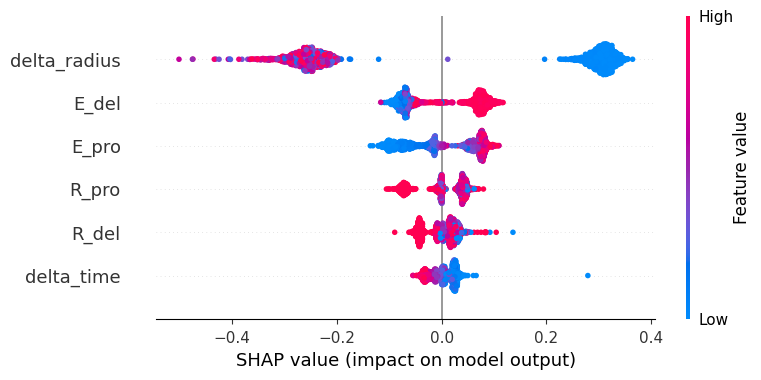
\includegraphics[width = 0.5\textwidth]{Images/Shap/summary_plot.png}
		\label{fig:summary_plot}
	}
	\subfloat[$\Delta t$ cut]{
		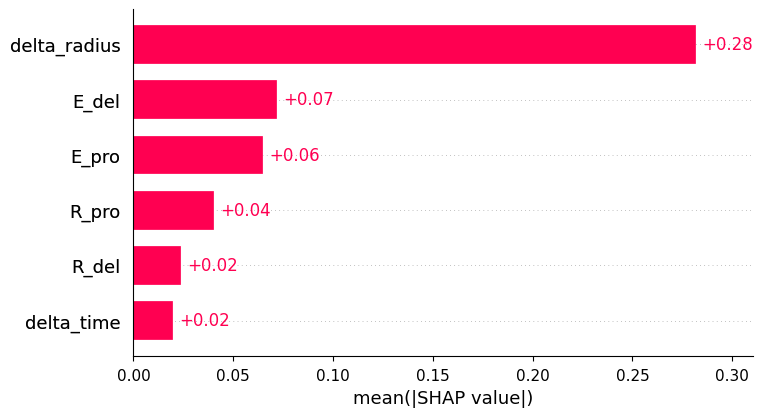
\includegraphics[width = 0.5\textwidth]{Images/Shap/feature_importance_bar.png}
	}
	
\end{figure}


The presented graphs depict the importance of each feature used by the algorithm for learning, measured by calculating the mean of the SHAP values. On the left, we see a histogram where the x-axis represents the mean absolute SHAP value for each feature. The first key characteristic of the model is evident here: the feature with the most importance in classification is $\Delta R$. Referring back to the graphs \ref{fig:hist_features}, it was already observable that $\Delta R$ is the feature that separates the IBD class most distinctly from the BKG class. A clear separation is evident from $2500 mm$ onwards, where BKG events prevail, while IBD events are more prevalent below $2500 mm$. 

The importance of this feature is further highlighted in the right-hand graph, where the x-axis represents the mean absolute SHAP value, and the y-axis represents the various features. Two distinct data clusters for the $\Delta R$ feature are clearly visible. For high values of this feature, the algorithm returns a negative SHAP value, which translates into identification as BKG events, as expected. For lower values of the feature, positive SHAP values are returned, corresponding to events correctly identified as IBD. It's also worth noting that the clusters are perfectly separated, indicating that the algorithm is very confident in labeling events based on this feature.

Second in order of importance, with a SHAP value approximately four times smaller than that of $\Delta R$, is "$E_{del}$", the energy of the delayed event, or electronic capture. Comparing with the feature histogram, it's clear that most BKG data occupy the initial part of the histogram, thus at lower energies, and the algorithm has learned to determine that for lower delayed signal energies, the event is classified as a BKG event. For slightly higher energies, given the presence of characteristic peaks that significantly increase the counts of IBD events, the algorithm learns to correctly determine an IBD event. 

Delving deeper into the analysis of this feature, a plot was created where the x-axis represents individual events, and the y-axis represents the effect that each event had on the $E_{del}$ feature. It is observed that for events in the range [1.9, 2.3] MeV and [4.9, 5.1] MeV, the algorithm has learned to perfectly distinguish the characteristic peaks of neutron capture compared to all background (BKG) events.

\begin{figure}[h!]
	\centering
	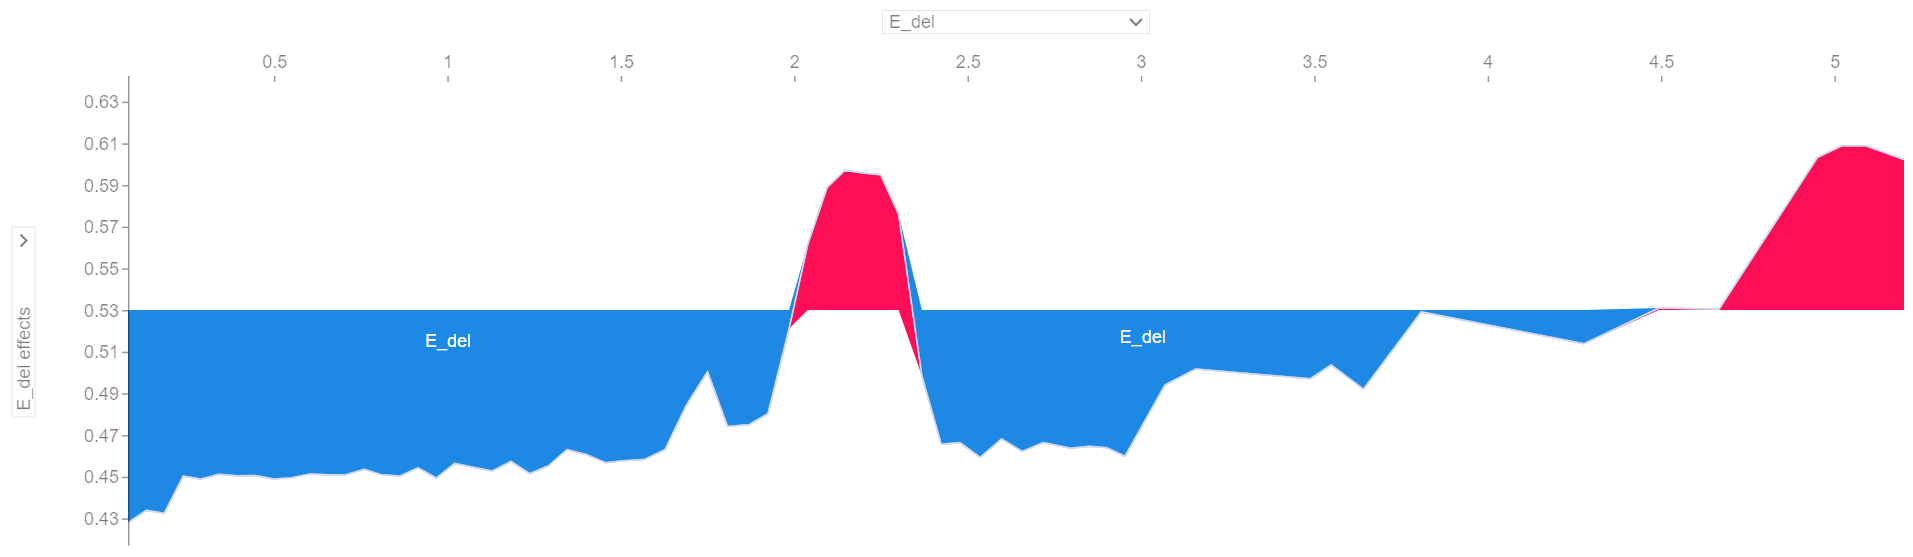
\includegraphics[width=\linewidth]{Images/Shap/E_del_force_plot.png}
	\label{fig:E_del_force_plot}
\end{figure}

Regarding the $E_{pro}$ feature, for values in the range [0, 1] MeV, the histogram is predominantly occupied by BKG events, and as seen from the summary plot, these are correctly identified by the algorithm. However, for prompt signals with energies within the positron-like spectrum, the algorithm identifies these events as IBDs. The features $R_{pro}$, $R_{del}$, and $\Delta t$ do not contribute significantly to the algorithm's ability to discern between the two classes from their distribution, as there are no clear differences between the feature histograms for IBD and BKG.

In conclusion, the SHAP values and the corresponding plots provide a valuable tool for understanding the decision-making process of the model, highlighting the importance of different features in the classification task. The model appears to perform well in distinguishing between IBD and BKG events, particularly using the $\Delta t$ and $E_{del}$ features. However, further analysis and improvements could be made, especially considering the features that currently contribute less to the classification.


\subsection{PyThorch}

\section{Conclusion}

% Please add the following required packages to your document preamble:
% \usepackage[table,xcdraw]{xcolor}
% If you use beamer only pass "xcolor=table" option, i.e. \documentclass[xcolor=table]{beamer}
\begin{table}[h!]
	\begin{tabular}{lllll}
		\cline{1-3}
		\multicolumn{1}{|l|}{} & \multicolumn{1}{c|}{{\color[HTML]{CE6301} \textbf{Manual Cut Algorithm}}} & \multicolumn{1}{l|}{{\color[HTML]{009901} \textbf{BDT Algorithm}}} &  &  \\ \cline{1-3}
		\multicolumn{1}{|l|}{\textit{Radioactivity}} & \multicolumn{1}{l|}{\begin{tabular}[c]{@{}l@{}}Efficiency: 99.9973\%\\ Purity: 100\%\end{tabular}} & \multicolumn{1}{l|}{\begin{tabular}[c]{@{}l@{}}Efficiency: 99.997684\%\\ Purity: 100\%\end{tabular}} &  &  \\ \cline{1-3}
		\multicolumn{1}{|l|}{\textit{True IBDs}} & \multicolumn{1}{l|}{\begin{tabular}[c]{@{}l@{}}Efficiency: 97.734\%\\ Purity:100\%\end{tabular}} & \multicolumn{1}{l|}{\begin{tabular}[c]{@{}l@{}}Efficiency: 99.997616\%\\ Purity: 100\%\end{tabular}} &  &  \\ \cline{1-3}
		&  &  &  & 
	\end{tabular}
\end{table}

